	
\chapter{Развој решења}

Циљ мастер рада био је \textit{истраживање могућности} примене алгоритама моделовања тема у основној верзији  при предлагању одговора на питање постављено природним језиком. Стога, алгоритам моделовања тема није развијан од почетка већ се користило готово решење у оквиру софтверског пакета \textit{Mallet}.
Основни разлог развоја софтверског окружења налази се у потреби тестирања различитих претпоставки везаних за примену алгоритама моделовања тема у задатом проблему. Стога је развојено, у програмској језику Java, неколико класа које су имале са циљ обезбеђивање лаког и једноставног тестирања претпоставки.

Анализа резултата тестирања хипотеза вршила се помоћу Matlab-а и  Microsoft Excel програма.
 
\section{Општи преглед пакета Mallet}

Софтверски пакет \textit{Mallet} је софтвер \textbf{отвореног кода - енг. open source} и представља скуп алгоритама машинског учења оријентисаних на текстуалне податке. Обухвата различите врсте алгоритама за  моделовања тема (енг. topic modeling), кластеровање (енг. clustering), класификацију (енг. classification), статистичке обраде природног језика (енг. statistical natural language processing) итд. Сви алгоритми развијени су у Java програмском језику

Алгоритам моделовања тема у овом пакету има две реализације. Основна верзија, која је коришћена у овом раду, представља имплементацију LDA-a (енг. Latent Dirichlet Allocation) Гибсовим узорковањем. Друга верзија предстваља хијерархијски LDA-a. Примена хијерархијске врста алгоритма моделовања тема није била предмет овог рада али би било интересантно испитати те могућности у будућем раду.

Софтверски пакет \textit{Mallet} може се користити на два начина : конзолно - коришћењем предефинисаних команди, или се, обзиром на то да је код јавно доступан, сам код може убацити у постојећи пројекат. Пошто је циљ истраживања био специфичан и захтевао извесне модификације основне верзије решења у пакету  \textit{Mallet}, у раду је коришћена друга опција.

 
\subsection{Подаци у Mallet-у}

 

\textit{Mallet} користи објекте класе \textbf{Instance} за представљање података при чему  сваки засебан објекат  представља посебан документ. У конкретном случају под \textbf{документом} се подразумева текст питања или одговора.  Дакле, један објекст класе \textbf{Instance}  представља или једно питање или један одговор.

Превођење "`сирових"' података у објекте класе  \textbf{Instance} представља предпроцесирање података за све алгоритме пакета \textit{Mallet} и неопходан је корак при коришћењу било ког од тих алгоритама. 

Превођење података у објекте класе \textbf{Instance}, обзиром на конструкторе, могло би да се посматра као тривијалан посао. Међутим, обзиром на специфичне захтеве исраживања, потребно је укључити и све кораке предпроцесирања који су наведени у претходом поглављу. За тако нешто је коришћена класа \textit{Pipe}, такође из пакета \textit{Mallet}.

\textit{Pipe} је апстрактна класа и представља надкласу за све класе које се користе за модификовање објекста  класе \textbf{Instance} у предпроцесирању. У пакету \textit{Mallet} постоји неколико предефинисаних класа које врше неке од трансформација поменутих у претходном поглављу - нпр. уклањање HTML ознака (класа CharSequenceRemoveHTML), превођење у мала слова ( класа  CharSequenceLowercase() ), формирање токена од текста (класа CharSequence2TokenSequence )  или уклањање често коришћених речи ( класа TokenSequenceRemoveStopwords ).
Поред поменутих, већ уграђених класа, за потребе рада дописане су још и :
\begin{itemize}
\item класа за уклањање наставака речи - PipeStem
\item класа за свођење на коренску реч - StanfordLemmatizer
\item класа за убацивање синонима - InsertSynonyms
\end{itemize}

У додатку су дате неке од тих класа.

Пошто предпроцесирање најчешће захтева више од једне трансформације, пракса је формирање низа објеката типа \textit{Pipe} који секвенцијално врше трансформацију објекта класе \textbf{Instance}. Тај низ најчешће се формира објекстом класе \textit{SerialPipe}.

Обзиром на то да улазни подаци у било који алгоритам машинског учења најчешће нису поједнични документи већ скупови документа, од интереса је и класа  \textit{InstanceList} којом се једноставно  апстрахује  скуп докумената. Објекти ове класе садрже групу\textbf{Instance} објеката над којима су извршене исте трансформације (исти SerialPipe).

\subsection{Алгоритам моделовања тема у Mallet-у }

Алгоритам моделовања тема у Mallet-у представља имплементацију LDA-а (Latent Dirichlet Allocation) преко Гибсовог узорковања. Постоји више имплементација од којих је \textit{ParallelTopicModel} најјефикаснија. У тој класи је реализован основни LDA-а алгоритам коришћењем Гибсовог узорковања. Перформансе су повећане паралелизацијом преко нити. Овај класа је коришћена у истраживању.

При моделовању тема следећи параметри су од интереса :

\begin{itemize}
\item број тема
\item број итерација
\item хиперараметри
\end{itemize}

Вредности ових параметара се задају пре моделовања тема и од њих директно зависи решење. 
У истраживању највећи акцент је био на проналажењу оптималних вредности ових параметара и то пре свега броја тема и итерација. Вредности хиперпараметара су фиксиране тако да, што  релистичније описију знања о полазном скупу података. То подразумева подједнаку вероватноћу свих тема у оквиру докумената као и подједнаку вероватноћу свих речи у оквиру свих тема. 

Приликом проналажење оптималне вредности броја тема и итерација прибегло се похлепном решењу тј. испитивању свох могућих комбинација. Разлог за такав приступ, поред проналажења оптималних вредности параметара, био је и испитивање \textbf{тренда} перформанси модела.   Обзиром да је то временски изузетно захтеван посао, овај део истраживања одрађен је коришћењем \textbf{кластера}. У додатку је пример скрипте којом се покрећу послови на кластеру. 

Процес моделовања тема извршава се у оквиру методе \textit{estimate} класе ParallelTopicModel где се, у одређеном броју итерација, врши Гибсово узороковање по познатим обрасцима. Овај процес још се назива и \textbf{тренирање модела}. Крајњи резултат представља \textbf{истрениран модел} који у себи садржи информације о :
\begin{itemize}
\item расподели тема унутар сваког документа
\item расподели речи унутар сваке теме
\end{itemize}


Једна од интересантних ствари које се на основу ових информација могу закључити је и расподела тема унутар \textbf{новог} документа тј. документа који није коришћен при тренирању. То се постиже класом \textit{TopicInferencer} која симулира  у одређеном броју итерација претходни процес тренирања, стим што се промене односе само на нови документ. Дакле, овим није могуће накнадно тренирати већ истрениран модел, али је из података истренираног модела могуће наслутити расподелу тема на невиђеном документу.

Поред наведене класе, у Mallet-у постоји и \textit{SimpleLDA}  која такође имплементира LDA-а алгоритам коришћењем Гибсовог узорковања али у верзији која није оптимизована. Због бољег разумевања суштине рада алгоритма, у почетној фази истраживања коришћена је ова класа. Касније се због перформанси прешло на решење у оквиру класе  ParallelTopicModel.


\section{Опис решења}

Основни циљ развоја софтвера био је селектовање одговора који најбоље одговара на постављено питање. Идеја решења је изградња \textbf{модела тема} над свим одговорима чиме би се добио истрениран модел који поседује знање о расподели тема над документима као и расподели речи унутар тема. Затим се за  постављено питање процењује расподела тема над њим и мери се \textbf{сличност} тог питања са свим одговорима у бази. Најсличнији одговор се проглашава одговором на постављено питање, при чему се кориснику предлаже 30 највероватнијих одговора.

У улазне податке спадају листа питања и листа одговора на та питања. Дакле, зна се који одговор припада ком питању, односно може се установити да ли је програм адекватно проценио који је прави одговор. Стога се за оцену квалитета решења може узети \textbf{број тачних одговора} који су се јавили у првих 10, 20 или 30 предложених. 

За мерење сличности питања и одговора коришћено је неколико метода :

\begin{itemize}
\item Косинусна сличност расподеле по темама - ово је најједноставнија мера сличности. Пошто је познат број тема, сваки документ се може представити вектором дужине броја тема. На $i-том$ месту у сваком вектору налази се вероватноћа, односно присуство $i-те$ теме у том документу. Косинусна сличност овакава два вектора представља меру сличности одговарајућих докумената. Што су расподеле по темама сличније, то ће мера сличности бити ближа 1. Основни разлог за овакво решење била је претпоставка да су питање и прави одговор \textbf{тематски} јако слични

\item Сума косинусних сличности расподела речи - обзиром да је позната расподела речи по темама могуће је  за сваку тему формирати вектор који за сваку реч из документа садржи вероватноћу те речи у одговарајућој теми. На овај начин се формирају два вектора, један за питање а други за одговор. Косинусна сличност ових вектора рачуна се за сваку тему а њихова сума представља меру сличности докумената

\item Вероватноћа генерисања питања на основу одговора и њене варијације - обзиром да је позната расподела тема по документима као и расподела речи унутар тема, једноставно се може прерачунати вероватноћа генерисања текста питња на основу текста одговора. Та вероватноћа представља меру сличности ова два документа.Варијације ове теме односе се на прерачунавање вероватноће. У раду су испитана још два додатна начина али је основна верзија показала најбоље резултате.

\end{itemize}

Испитане мере сличности разликују се по прецизности, брзини рада и меморијским захтевима. Испоставило се да су  за примену на већи скуп података погодна прва и трећа ( са варијантама) метода .

Идејни ток решења може се представити  дијаграмом као на слици 6.1:

\begin{figure}[H]
    \centering
   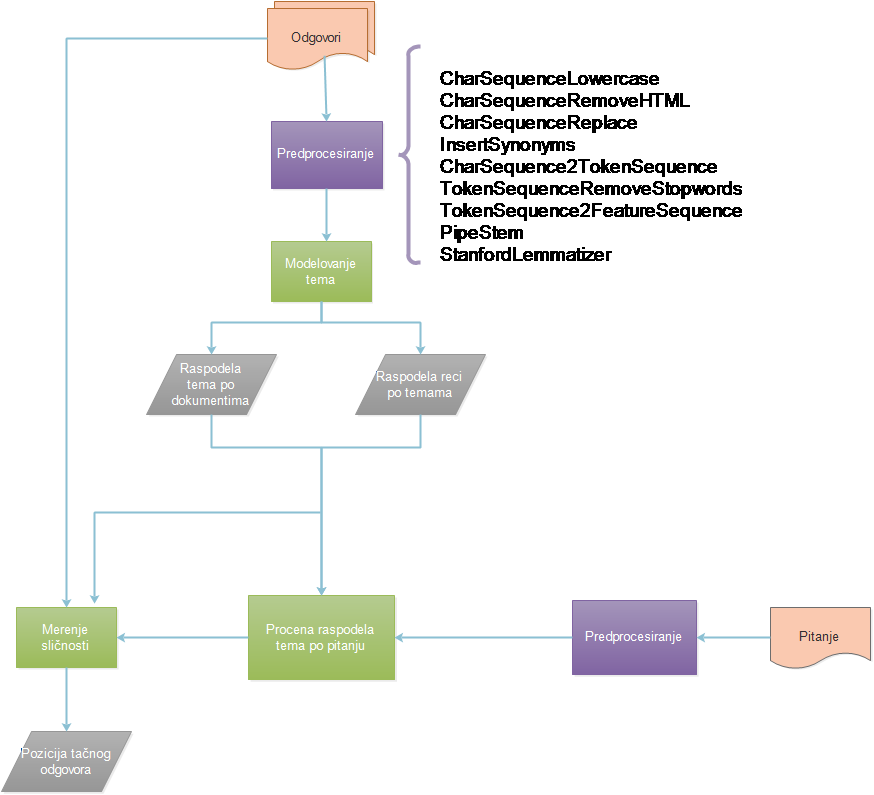
\includegraphics[scale=0.7]{./Slike/slika38.png} 
	\caption{Ток решења}
	\label{fig:slika1}
\end{figure}


Важно је приметити да се у предпроцесирању не морају извршити све наведене трансформације нити у назаначеном редоследу. Одабир подскупа транформација директно утиче на резулат док редослед извршавања мора имати смислени ток. У конкретном истраживању, наведене трансформације су извршаване у датом редоследу. Главни циљ је био испитивање утицаја синонима, стеминга и лемитизације на резултат, тако да су ове три транформације укљичиване и искључиване како би се испитале све могуће комбинације.

Исто тако, ради конзистентности решења, структура и редослед предпроцесирања питања и одговора морају бити \textbf{исти}. Из тог разлога су на дијаграму и обојени истом бојом.


